\documentclass{beamer}

\usepackage[utf8]{inputenc}
\usepackage{hyperref}

\usetheme{Berkeley}
\beamertemplatenavigationsymbolsempty
\setbeamertemplate{headline}{}
 
\title{Import Data from External Sources into FoodChain-Lab}
\date{}
 
\begin{document}
\maketitle

\section{Content}
\begin{frame}
	\begin{itemize}
		\item This tutorial shows how data can imported into FoodChain-Lab without using the Excel templates.
		\item Therefore the external data has to read into KNIME tables.
		\item KNIME provides a multitude of reader nodes for various data formats (e.g. csv, SQL databases, ...).
		\item Here we just show which tables are needed by FoodChain-Lab and which columns they must contain. To do so the we have created these tables with \textbf{Table Creator} nodes.
	\end{itemize}
\end{frame}
 
\section{1}
\begin{frame}
	\begin{center}
  		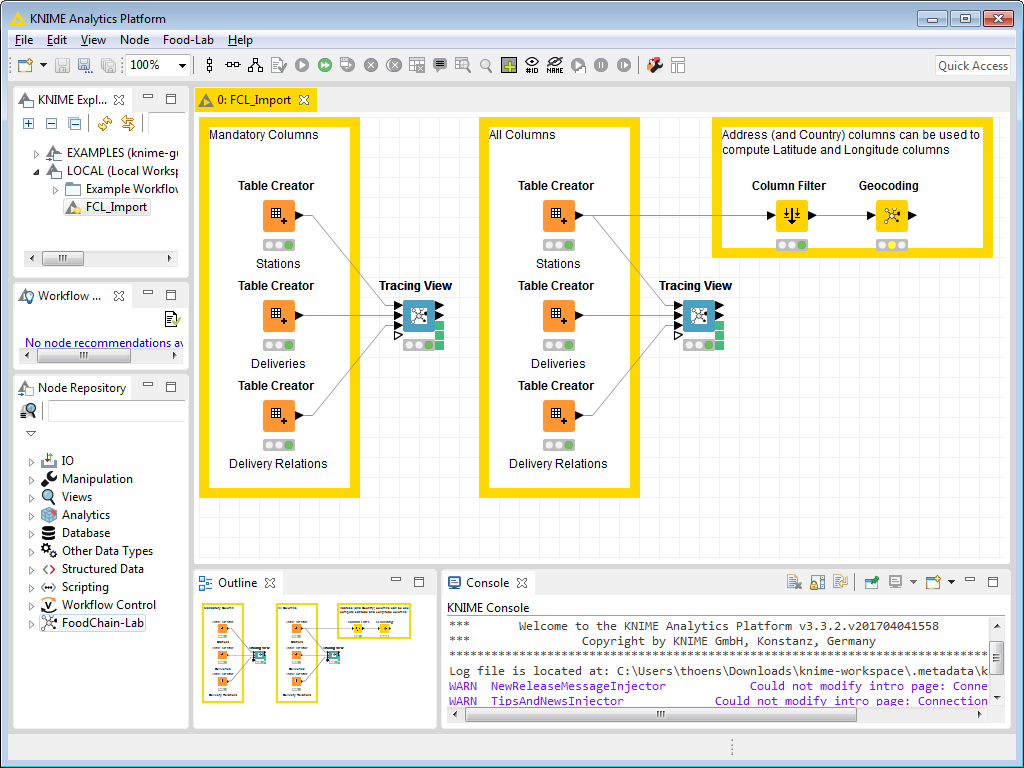
\includegraphics[height=0.6\textheight]{1.png}
	\end{center}
	\begin{itemize}
		\item Import the workflow from \url{https://github.com/SiLeBAT/BfROpenLabResources/raw/master/GitHubPages/workflows/FCL_Import.knwf}.
	\end{itemize}
\end{frame}

\section{2}
\begin{frame}
	\begin{center}
  		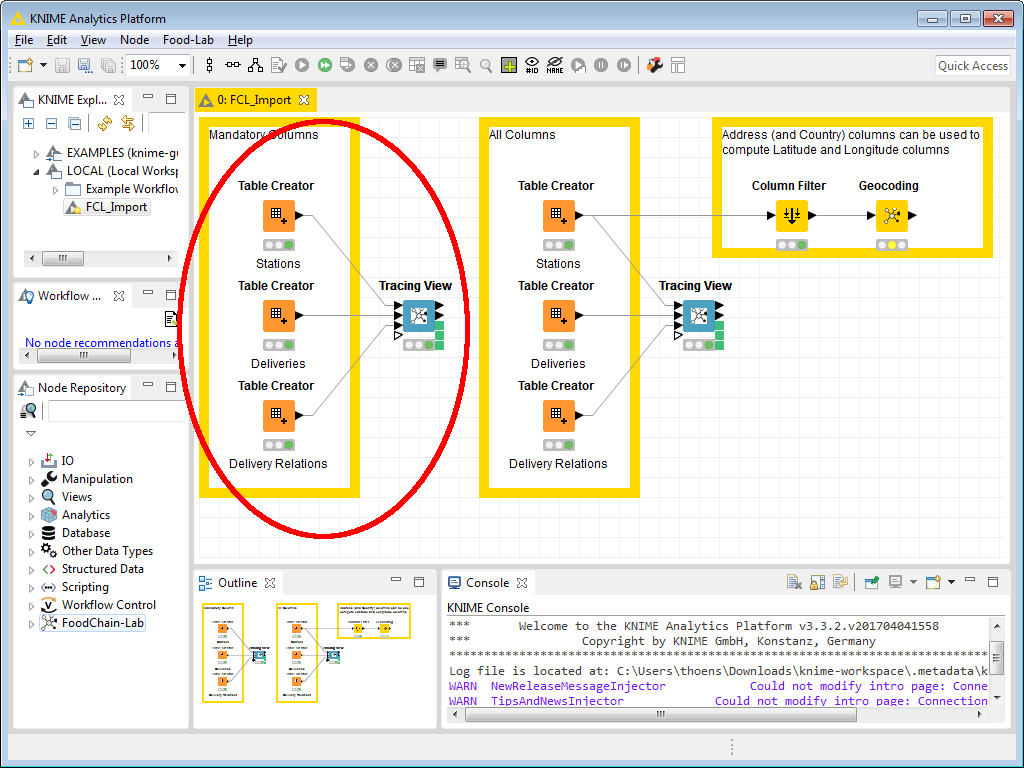
\includegraphics[height=0.6\textheight]{2.png}
	\end{center}
	\begin{itemize}
		\item FoodChain-Lab needs three tables to perform a tracing analysis: \textbf{Stations}, \textbf{Deliveries} and \textbf{Delivery Relations}.
		\item The \textbf{Table Creator} nodes on the left show all mandatory columns for these three tables.
	\end{itemize}
\end{frame}

\section{3}
\begin{frame}
	\begin{center}
  		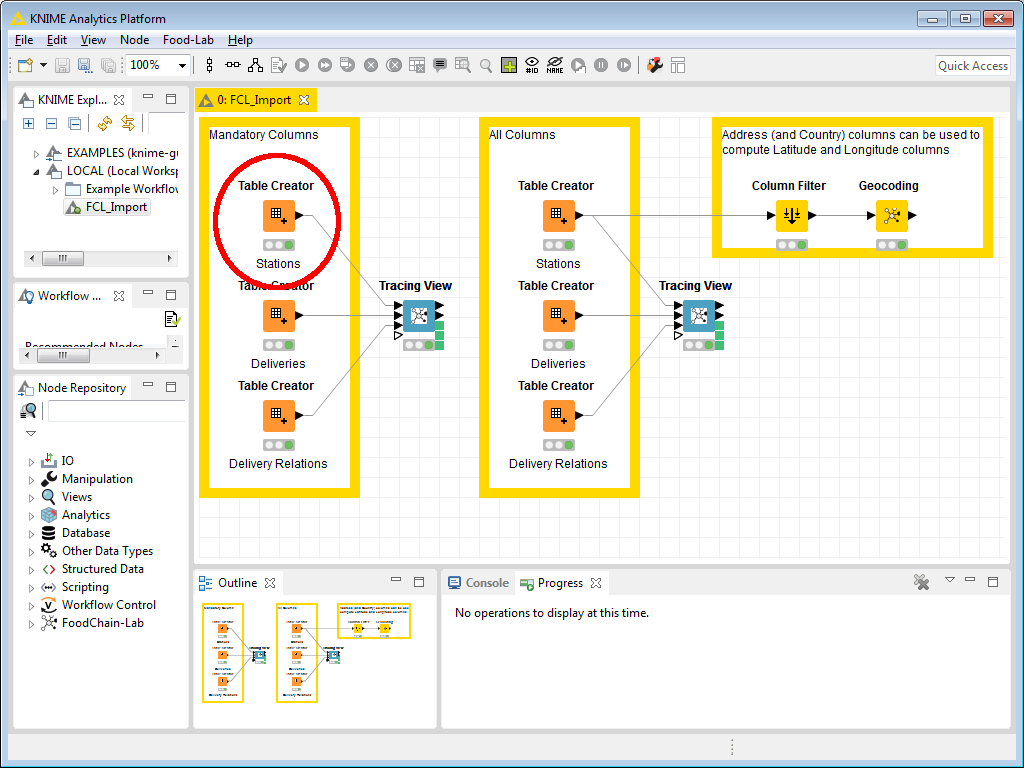
\includegraphics[height=0.6\textheight]{3.png}
	\end{center}
	\begin{itemize}
		\item Double click on the \textbf{Table Creator} for the \textbf{Stations} table to open its dialog.
	\end{itemize}
\end{frame}

\section{4}
\begin{frame}
	\begin{center}
  		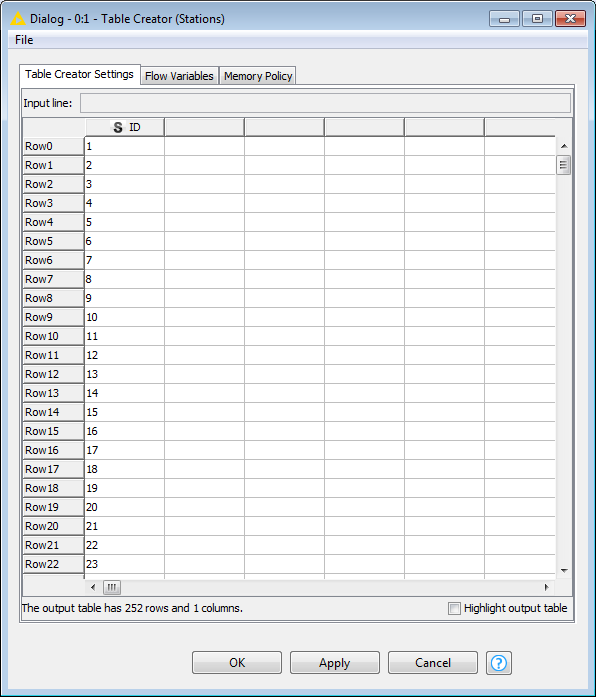
\includegraphics[height=0.6\textheight]{4.png}
	\end{center}
	\begin{itemize}
		\item As you can see the only mandatory column in the \textbf{Stations} table is the column \textbf{ID} of type string.
	\end{itemize}
\end{frame}

\section{5}
\begin{frame}
	\begin{center}
  		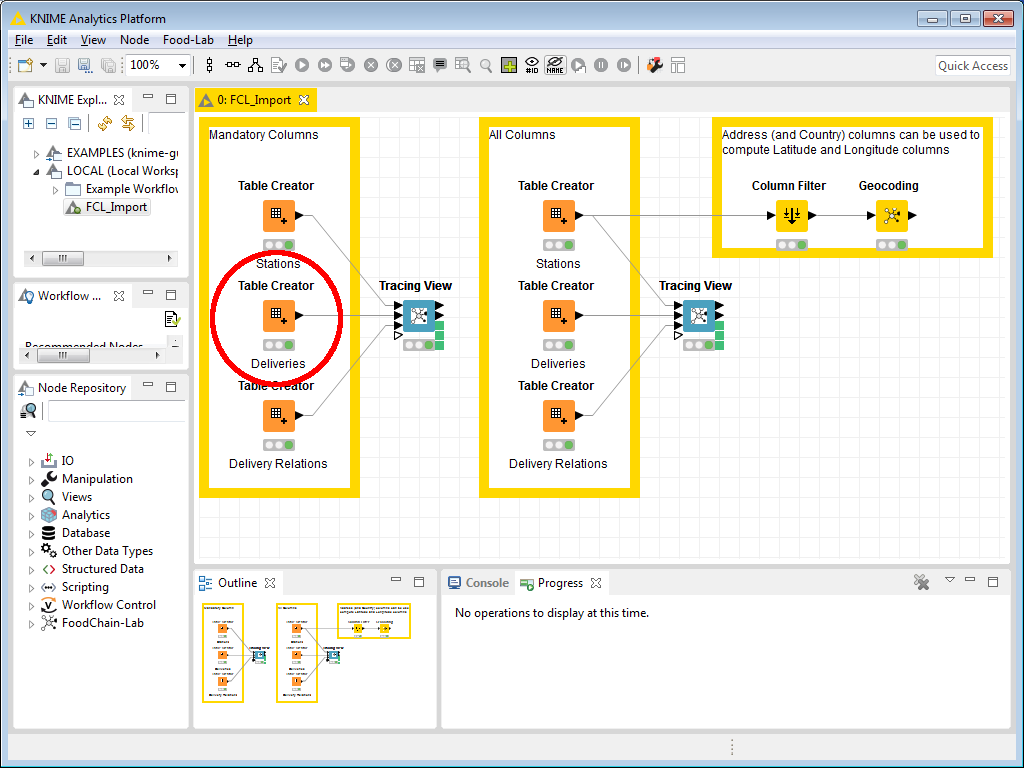
\includegraphics[height=0.6\textheight]{5.png}
	\end{center}
	\begin{itemize}
		\item Double click on the \textbf{Table Creator} for the \textbf{Deliveries} table to open its dialog.
	\end{itemize}
\end{frame}

\section{6}
\begin{frame}
	\begin{center}
  		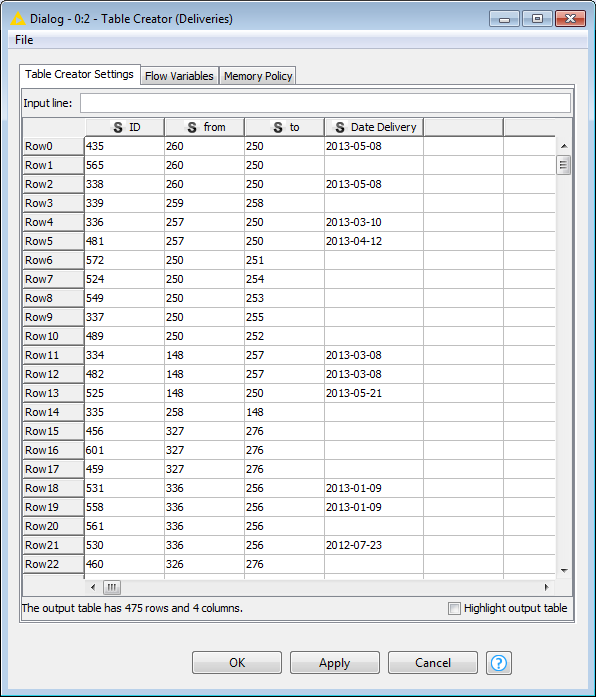
\includegraphics[height=0.6\textheight]{6.png}
	\end{center}
	\begin{itemize}
		\item The \textbf{Deliveries} table has three mandatory columns: \textbf{ID}, \textbf{from} and \textbf{to} (all of type string)
		\item The \textbf{from} and \textbf{to} columns contain the source station and target station \textbf{IDs}.
	\end{itemize}
\end{frame}

\section{7}
\begin{frame}
	\begin{center}
  		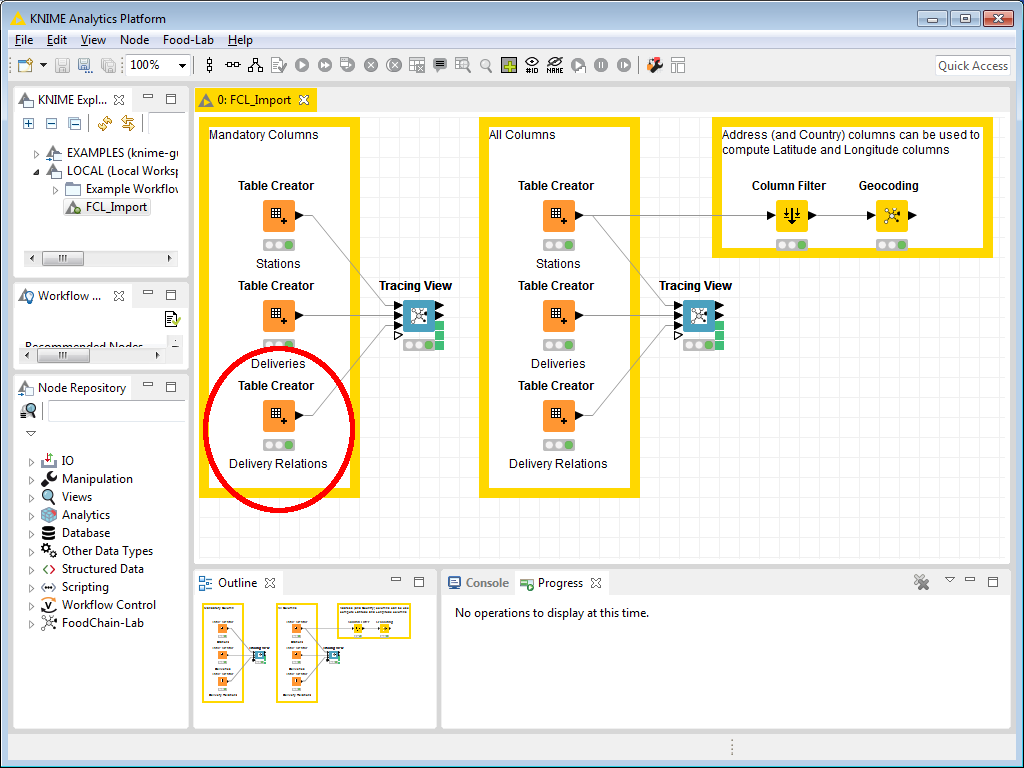
\includegraphics[height=0.6\textheight]{7.png}
	\end{center}
	\begin{itemize}
		\item Double click on the \textbf{Table Creator} for the \textbf{Delivery Relations} table to open its dialog.
	\end{itemize}
\end{frame}

\section{8}
\begin{frame}
	\begin{center}
  		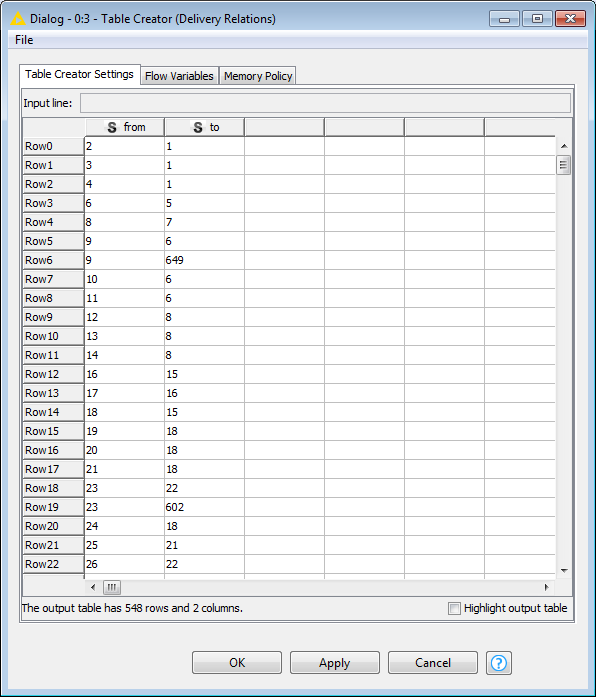
\includegraphics[height=0.6\textheight]{8.png}
	\end{center}
	\begin{itemize}
		\item The \textbf{Delivery Relations} table has the columns \textbf{from} and \textbf{to} of type string.
		\item These columns contain \textbf{IDs} from the \textbf{Delivery} table and are meant to connect two deliveries.
		\item The \textbf{from}-delivery is a part/ingredient of the \textbf{to}-delivery. A contamination can spread from "\textbf{from}" to "\textbf{to}".
	\end{itemize}
\end{frame}

\section{9}
\begin{frame}
	\begin{center}
  		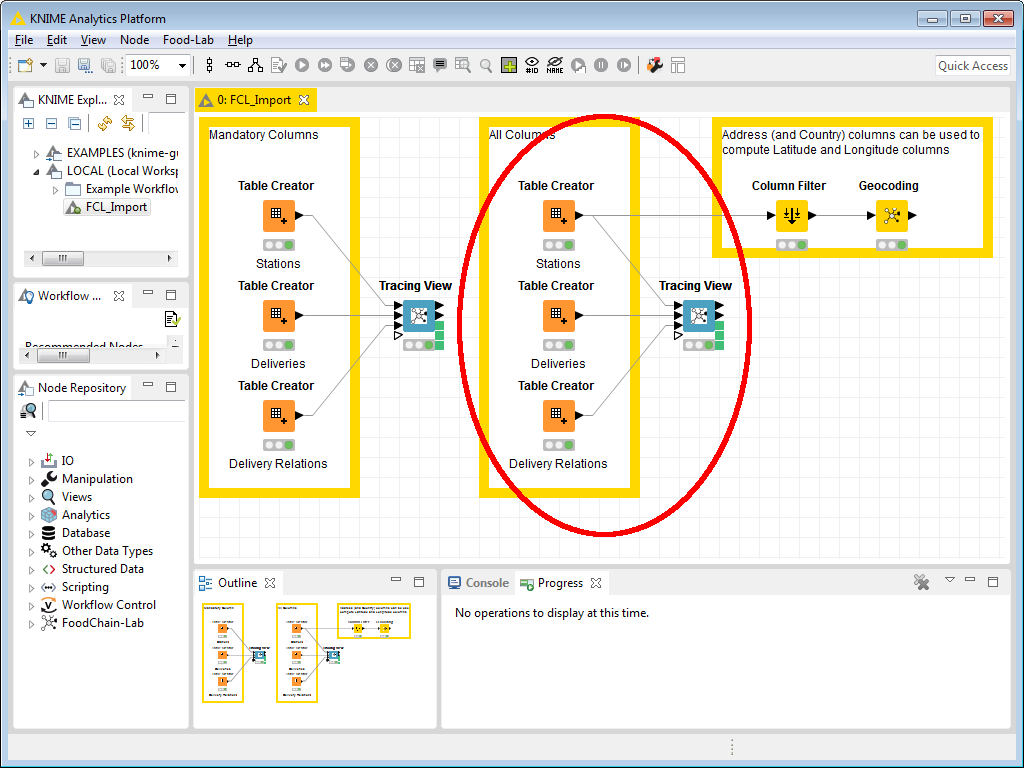
\includegraphics[height=0.6\textheight]{9.png}
	\end{center}
	\begin{itemize}
		\item Now we will look the \textbf{Table Creator} nodes on the right which show the optional columns for the three tables.
	\end{itemize}
\end{frame}

\section{10}
\begin{frame}
	\begin{center}
  		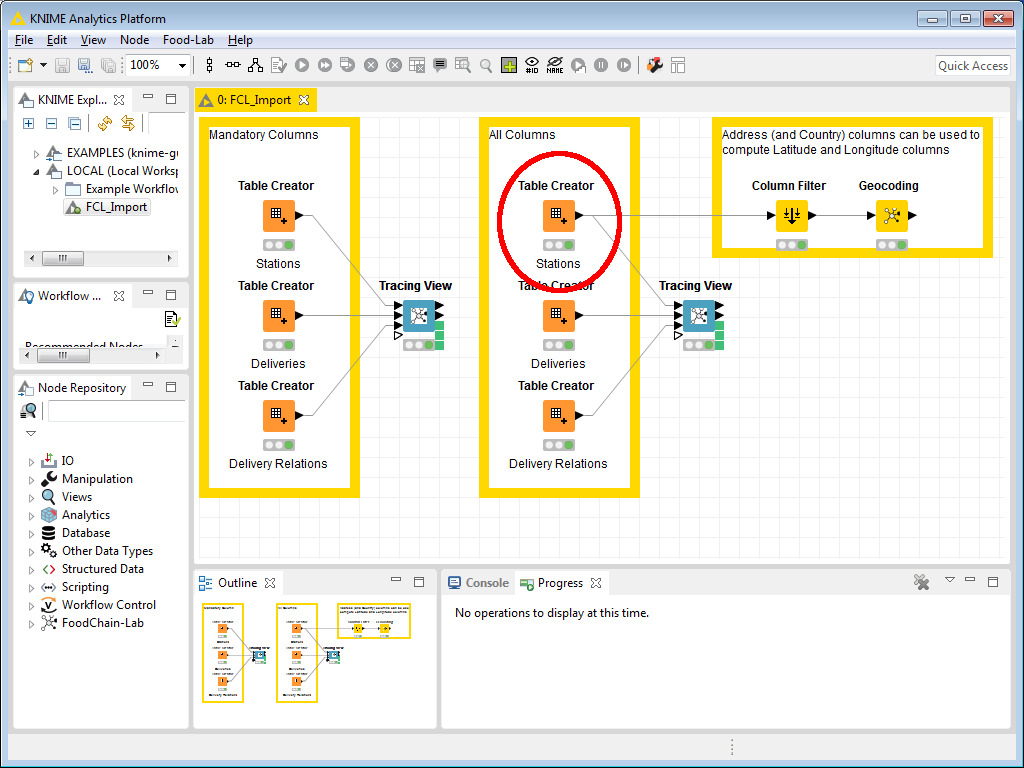
\includegraphics[height=0.6\textheight]{10.png}
	\end{center}
	\begin{itemize}
		\item Double click on the \textbf{Table Creator} for the \textbf{Stations} table to open its dialog.
	\end{itemize}
\end{frame}

\section{11}
\begin{frame}
	\begin{center}
  		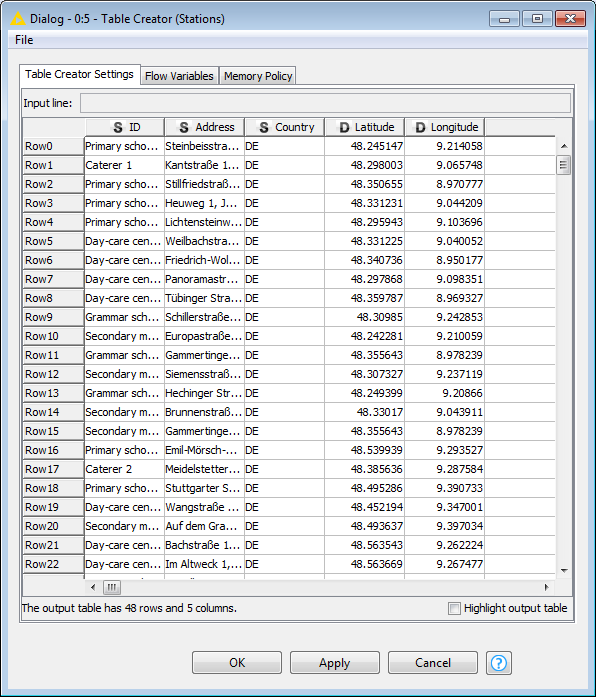
\includegraphics[height=0.5\textheight]{11.png}
	\end{center}
	\begin{itemize}
		\item The optional columns for the \textbf{Stations} table are \textbf{Address}, \textbf{Country}, \textbf{Latitude} and \textbf{Longitude}.
		\item \textbf{Latitude} and \textbf{Longitude} are used for the geographical visualization in the \textbf{Tracing View} and \textbf{Address} and \textbf{Country} can be used for geocoding, if \textbf{Latitude} and \textbf{Longitude} are not known yet.
		\item Any other arbitrary columns of this table can also be used in the \textbf{Tracing View} for highlighting etc.
	\end{itemize}
\end{frame}

\section{12}
\begin{frame}
	\begin{center}
  		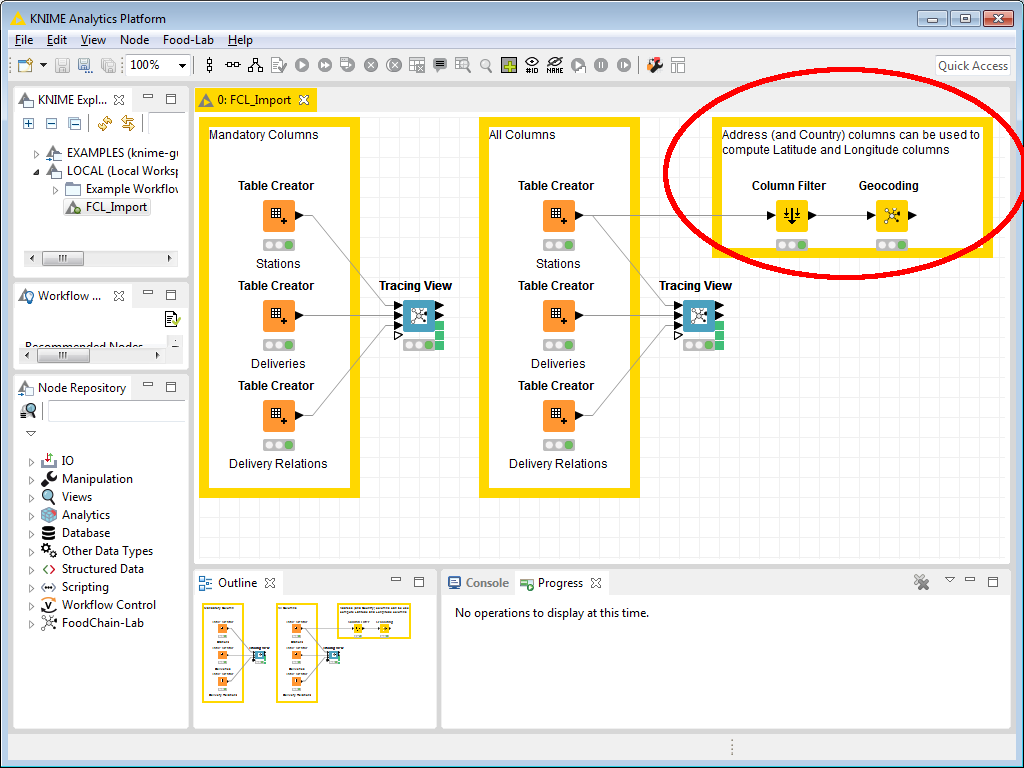
\includegraphics[height=0.6\textheight]{12.png}
	\end{center}
	\begin{itemize}
		\item The \textbf{Geocoding} node in the upper right corner shows how \textbf{Address} and \textbf{Country} can be used for geocoding to compute \textbf{Latitude} and \textbf{Longitude}.
	\end{itemize}
\end{frame}

\section{13}
\begin{frame}
	\begin{center}
  		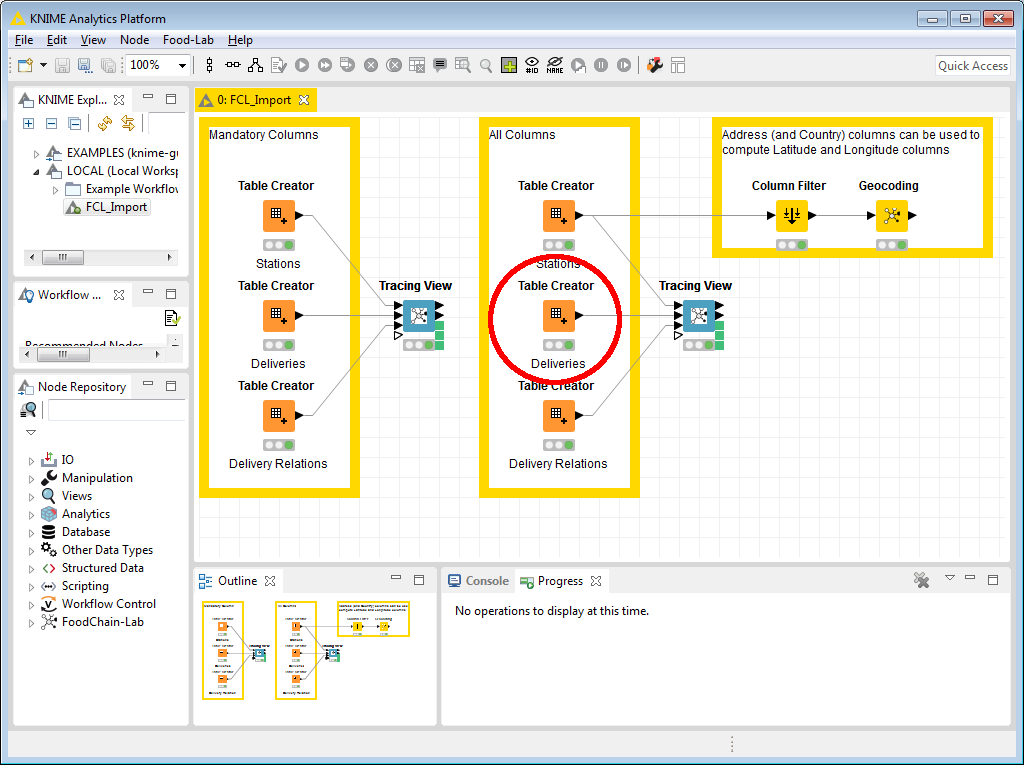
\includegraphics[height=0.6\textheight]{13.png}
	\end{center}
	\begin{itemize}
		\item Double click on the \textbf{Table Creator} for the \textbf{Deliveries} table to open its dialog.
	\end{itemize}
\end{frame}

\section{14}
\begin{frame}
	\begin{center}
  		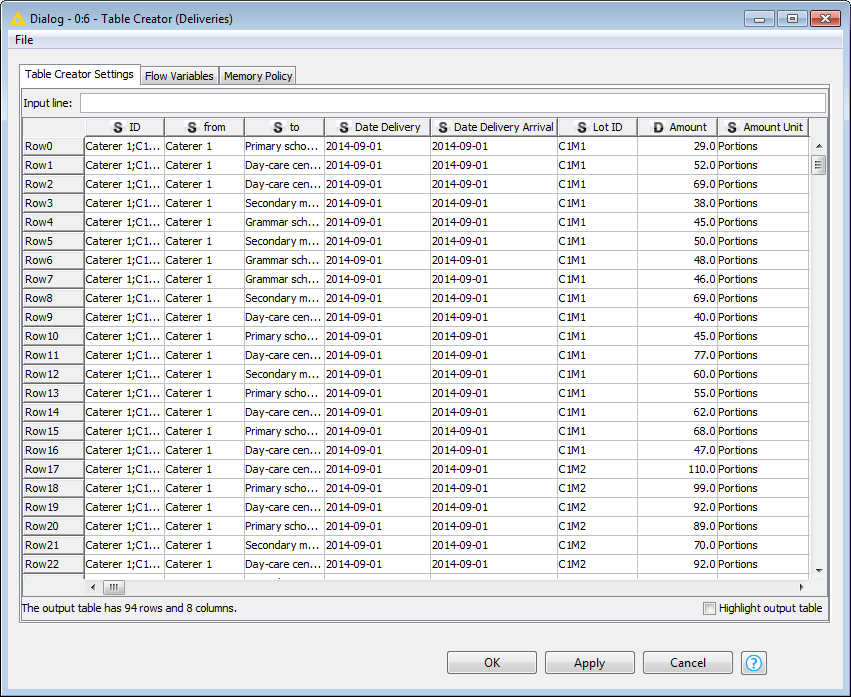
\includegraphics[height=0.45\textheight]{14.png}
	\end{center}
	\begin{itemize}
		\item The optional columns are \textbf{Date Delivery}, \textbf{Date Delivery Arrival}, \textbf{Lot ID}, \textbf{Amount} and \textbf{Amount Unit}.
		\item The date columns are of type string and in YYYY-MM-DD format. They used for computing cross contamination.
		\item If the \textbf{Lot ID} column (of type string) is provided, lot-based scores are computed.
		\item The amount columns are just used for plausibility checks.
		\item Any other arbitrary columns of this table can also be used in the \textbf{Tracing View} for highlighting etc.
	\end{itemize}
\end{frame}

\section{15}
\begin{frame}
	\begin{center}
  		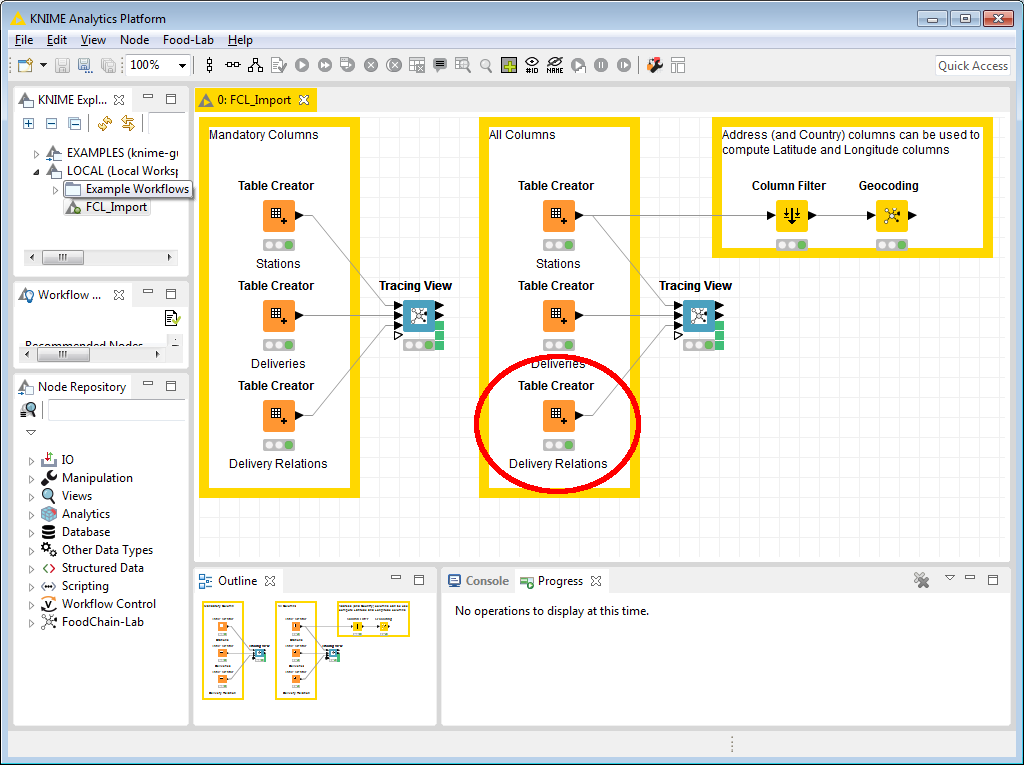
\includegraphics[height=0.6\textheight]{15.png}
	\end{center}
	\begin{itemize}
		\item Double click on the \textbf{Table Creator} for the \textbf{Deliveries Relations} table to open its dialog.
	\end{itemize}
\end{frame}

\section{16}
\begin{frame}
	\begin{center}
  		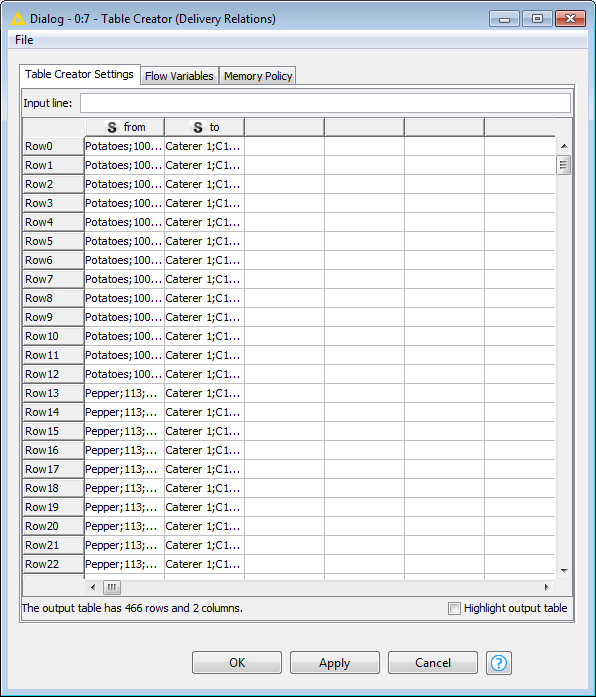
\includegraphics[height=0.6\textheight]{16.png}
	\end{center}
	\begin{itemize}
		\item The \textbf{Delivery Relations} table does not have any optional columns.
		\item All columns other than \textbf{from} and \textbf{to} are ignored.
	\end{itemize}
\end{frame}

\end{document}